\documentclass{article}
\usepackage{amsmath}
\usepackage{amssymb}
\usepackage[svgnames]{xcolor}
\usepackage{graphicx}
\usepackage{enumitem}
\usepackage{multicol}
\usepackage{bbm}

\title{Computer Graphics: Assignment 03} % Title

\author{Lina Gundelwein, Letitia Parcalabescu, Anushalakshmi Manila} % Author name

\date{\today} % Date for the report

\begin{document}

\maketitle 

\section*{3. Transformations} 

A and B are both scaling-mirroring matrices. \\
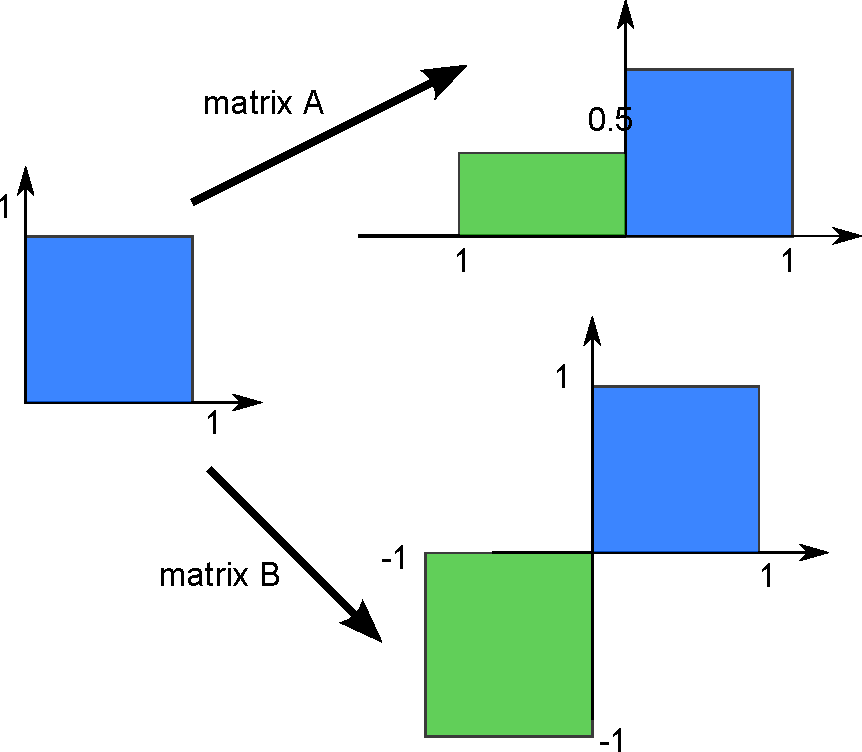
\includegraphics[width=0.5\linewidth]{drawing} \\

\begin{itemize}
\item Rotating an object without translating it equals a translation around the coordinate center.
\item Rotating after translating the center of the rectangle to zero results in a rotation around the rectangle center. (And a translation of (-3,2) if there is it is not translated back afterwards).
\item Rotating after tranlation of $V_1$ to the coordinate center will result in the rectangle rotated around $V_1$ and shifted by (-2,2).
\item Yes it is possible if you work with homogeneous coordinates. Transform vertices to homogeneous coordinates ($(2,2) \rightarrow (2,2,1)$ etc.) and multiply with matrix
\begin{equation*}
P = 
\begin{pmatrix}
1 & 0 &2\\
0 & 1 & 2\\
0 & 0 & 1
\end{pmatrix}
\begin{pmatrix}
\frac{\sqrt{2}}{2} & - \frac{\sqrt{2}}{2} & 0\\
\frac{\sqrt{2}}{2} &  \frac{\sqrt{2}}{2} & 0\\
0 & 0 & 1
\end{pmatrix}
\begin{pmatrix}
1 & 0 &-2\\
0 & 1 &-2\\
0 & 0 & 1
\end{pmatrix}=
\begin{pmatrix}
\frac{\sqrt{2}}{2} & - \frac{\sqrt{2}}{2} & 2\\
\frac{\sqrt{2}}{2} &  \frac{\sqrt{2}}{2} & 2-2\sqrt{2}\\
0 & 0 & 1
\end{pmatrix}\,.
\end{equation*}
\end{itemize}
\end{document}